\chapter{Planning}

\subsection{Planning fase overview}
\todo[inline]{Here we need an overview of the first planning fase}

\newpage
\input ch/planning/sec/wbs.tex

\newpage
\subsection{Gantt diagram}

A Gantt diagram is a representation of all the work hours, milestones and deadlines that is involved in a project. The Gantt diagram for our project is given in figure~\ref{fig:gantt}.

\begin{figure}[H]
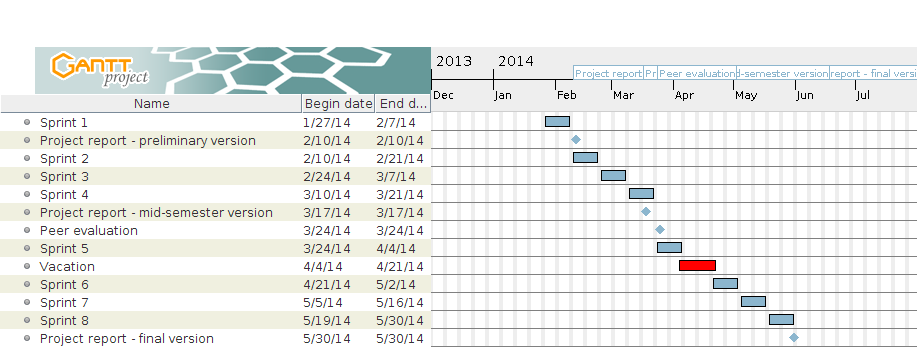
\includegraphics[width=\textwidth]{ch/planning/fig/gantt.png}
\caption{The Gantt diagram with sprints and milestones.}
\label{fig:gantt}
\end{figure}

\input ch/planning/sec/agileDevelopment.tex
\input ch/planning/sec/scrum.tex
\input ch/planning/sec/extremeProgramming.tex

\input ch/planning/sec/risk.tex
%\input ch/planning/sec/architecture.tex
